\nonstopmode
\documentclass{article}

\usepackage[utf8]{inputenc}
\usepackage{geometry}
\usepackage{graphicx}
\usepackage{polski}
\usepackage{subcaption}

\graphicspath{ {images/} }
\geometry{legalpaper, portrait, margin=1in}

\title{\LARGE Algorytmy grafowe\\ Sprawozdanie nr 3}
\author{Adam Piaseczny \\	151757 \and
				Igor Szczepaniak \\ 151918}
\date{Grupa piątkowa 11:45}

\begin{document}

\maketitle
\pagebreak

\tableofcontents
\pagebreak

\section{Wprowadzenie}

W tym sprawozdaniu zbadaliśmy sposoby analizy grafów i ich reprezentacji maszynowych, byliśmy w stanie dzięki temu zweryfikować wiadomości poznane w trakcie zajęć. Kod źródłowy został napisany w języku \textbf{python} ze względu na prostotę implementacji.

Zaimplementowaliśmy metodę sortowania topologicznego działającą w dwóch wyodrębnionych etapach: obliczającą dla każdego wierzchołka etykiety czasowe rozpoczęcia i zakończenia analizy oraz sprawdzającą acykliczność przez zliczanie łuków powrotnych. Wygenerowaliśmy 10 losowych grafów skierowanych $G=(V,A)$ o rożnych $|V|=n$.

\section{Obliczanie etykiet czasowych w zależności od gęstości grafu}

Etykiety czasowe to dwie unikalne wartości przydzielane każdemu wierzchołkowi oznaczające czas, w którym dany wierzchołek został włożony na stos, oraz z niego zdjęty podczas działania algorytmu DFS (Depth First Search, czyli wyszukiwanie "w głąb"). Algorytm działa w następujący sposób:

\begin{enumerate}
\item Zaczynamy algorytm na dowolnym nieodwiedzonym wierzchołku w grafie.
\item Dokładamy wierzchołek na stos
\item Znajdujemy pierwszego nieodwiedzonego następnika, jeśli go nie ma - zdejmujemy ten wierzchołek ze stosu
\item Wykonujemy kroki 2-4 dla każdego wierzchołka na szczycie stosu do momentu wyczerpania stosu. Jeśli po wyczerpaniu stosu graf dalej posiada wierzchołki nieodwiedzone, uruchamiamy DFS ponownie.
\end{enumerate}

Złożoność algorytmu DFS to $O(n+m)$, gdzie $n$ to liczba wierzchołków w grafie, a $m$ to łączna ilość łuków. Dodatkowym nakładem czasowym przy wykonywaniu DFS jest sprawdzanie następników danego wierzchołka - czas tej operacji jest uzależniony od wybranej reprezentacji maszynowej grafu. Tworząc algorytm zliczający etykiety czasowe zauważyliśmy, że najbardziej trafną reprezentacją przy naszym zastosowaniu jest \textbf{lista następników}. Struktura ta działa w następujący sposób:

\begin{enumerate}
\item Tworzymy tablicę o szerokości $n$ elementów, gdzie $n$ to liczba wierzchołków
\item Do każdej komórki w tablicy wstawiamy listę następników dla danego wierzchołka
\end{enumerate}

Ta reprezentacja pozwala na szybsze wyszukiwanie następników niż w macierzy sąsiedztwa, z racji ograniczenia ilości operacji do minimum. Lista następników posiada złożoność od $O(1)$ do $O(n)$ i była bardzo prosta do implementacji w języku \textbf{python}.

Najgorszą reprezentacją grafu dla wyszukiwania następnika jest macierz incydencji, gdzie aby znaleźć następnika dla danego wierzchołka trzeba liczyć się z czasem rzędu $O(n\times m)$, więc im większa jest gęstość grafu, tym mniej korzystna jest ta reprezentacja. Gęstość grafu $d$ jest stosunkiem liczby łuków w danym grafie do największej możliwej liczby łuków (w grafie pełnym). Każdy nasz test spełniał zależność $m>n$, gdzie $m=d\times n\times (n-1)$ .

W następującej tabeli przedstawiliśmy przy dwóch gęstościach zależność czasu trwania etapu obliczania etykiet czasowych od liczby wierzchołków $n$.

\begin{figure}[h]
\centering
  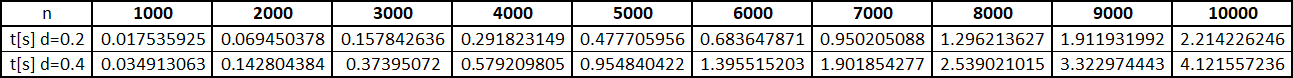
\includegraphics[width=1.0\linewidth]{etykiety_tabela}
	\captionof{figure}{Obliczanie etykiet (tabela)}
  \label{fig:etykiety_tabela}
\end{figure}%

Z wyników z stworzyliśmy następujący wykres:

\begin{figure}[h]
\centering
  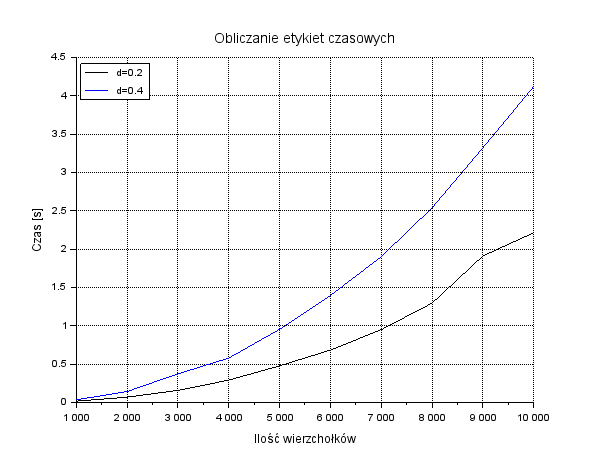
\includegraphics[width=0.5\linewidth]{etykiety}
	\captionof{figure}{Obliczanie etykiet}
  \label{fig:etykiety}
\end{figure}%

Test obliczania etykiet czasowych został wykonany na liście następników. Można zaobserwować, że wraz ze wzrostem gęstości czas na obliczanie wszystkich etykiet również rośnie, dzieje się tak ponieważ gęstość wpływa na średnią ilość następników danego wierzchołka. Zwiększona gęstość grafu najbardziej wpływa na czas działania algorytmu przy reprezentacji, gdzie wyszukiwanie następnika zależy w dużym stopniu od ilości łuków. Reprezentacje, które są wrażliwe na gęstość to między innymi:

\begin{itemize}
\item Lista łuków - $O(m)$
\item Lista poprzedników - $O(n+m)$
\item Macierz incydencji - $O(n\times m)$
\end{itemize}

Macierz sąsiedztwa jest niewrażliwa na ilość istniejących łuków z racji czasu wyszukiwania następnika od $O(1)$ do $O(n)$, w tej strukturze zmiana gęstości grafu jest najmniej widoczna przy stałych wartościach $n$.

\section{Zliczanie łuków powrotnych}

Zliczanie łuków powrotnych w przypadku naszego zastosowania odbywa się używając etykiet czasowych obliczanych przy przejściu algorytmu DFS - $d[v]$ jest etykietą startową analizy, a $f[v]$ jest etykietą zakończenia analizy. Sprawdzanie, czy dany łuk $(u,v)\in A$ jest powrotny wiąże się ze spełnieniem poniższej zależności: $d[v] < d[u] < f[u] < f[v]$. Jeśli ta zależność jest prawdziwa dla analizowanego łuku - wiemy, że jest on powrotny.

W poniższej tabeli przedstawiliśmy liczbę łuków powrotnych dla poszczególnych liczby wierzchołków $n$ oraz gęstości $d$.

\begin{figure}[h]
\centering
  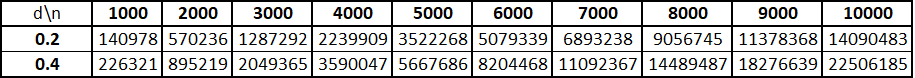
\includegraphics[width=1.0\linewidth]{luki_tabela.png}
	\captionof{figure}{Zliczanie łuków (tabela)}
  \label{fig:luki_tabela}
\end{figure}%

Nasz eksperyment wykazał znaczącą ilość łuków powrotnych w każdym grafie, przez co żaden graf analizowany podczas eksperymentu nie był acykliczny, co jest warunkiem koniecznym do sortowania topologicznego.

Jeśli uporządkujemy wierzchołki malejąco według etykiety zakończenia analizy $f[v]$ otrzymamy porządek topologiczny dla danego grafu skierowanego. Porządek topologiczny pozwala na ustalenie kolejności wykonywania operacji tak, aby nie doszło do kolizji - przykładowym zastosowaniem sortowania topologicznego jest unikanie konfliktów zależności przy instalowaniu wielu programów jednocześnie. W porządku topologicznym łuk powrotny jest łukiem, który dąży w odwrotnym kierunku do ustalonego i nie pozwala na praktyczne zastosowania takiego układu (w przypadku wcześniejszego przykładu zaszedłby konflikt zależności) - z tego powodu grafów cyklicznych nie można posortować topologicznie.

\section{Zliczanie łuków powrotnych dla różnych reprezentacji grafu}

W tym teście sprawdziliśmy zależność czasu trwania etapu zliczania łuków powrotnych dla 3 reprezentacji grafu: macierzy sąsiedztwa, listy następników oraz listy łuków. W naszej implementacji macierzy sąsiedztwa dla grafu skierowanego o wymiarze $n\times n$ wierzchołek o numerze wiersza jest poprzednikiem a wierzchołek o numerze kolumny jest następnikiem. Istnienie krawędzi między tymi dwoma wierzchołkami zaznaczane jest przez istnienie wartości 1 w danej komórce, w przeciwnym przypadku w komórce znajduje się wartość 0. Lista łuków jest natomiast tablicą dwuelementową, gdzie pierwszy element wstawiany to poprzednik, a drugi to następnik.

Operacją wykonywaną przy zliczaniu liczby łuków powrotnych jest sprawdzenie zbioru łuków. Najgorsza dla tej operacji jest macierz sąsiedztwa, w której zawsze musimy przejść całą macierz - jest to czas rzędu $O(n^2)$. Lista następników wykonuje tę operacje w czasie $O(n+m)$, jest przez to w dużym stopniu zależna od gęstości grafu. Najlepsza dla tej operacji jest lista łuków, gdzie cała lista jest zbiorem łuków. Reprezentacja ta również jest zależna od gęstości grafu, natomiast dzięki swojej złożoności $O(m)$ jest w stanie szybciej wykonać operację niż lista następników.

Otrzymane wyniki przedstawiliśmy poniżej w dwóch tabelach, dla różnych wartości $d$

\begin{figure}[h]
\centering
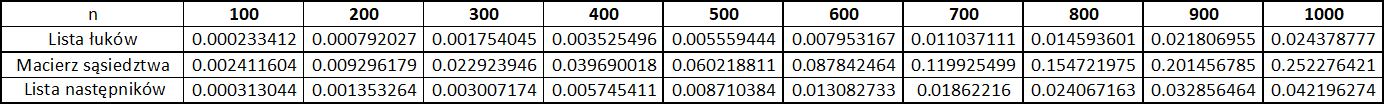
\includegraphics[width=1.0\linewidth]{luki_reprezentacje_tabela}
\captionof{figure}{$d=0.2$ Zliczanie łuków z 3 reprezentacji - tabela}
\label{fig:luki_reprezentacje_tabela}
\end{figure}%

\begin{figure}[h]
\centering
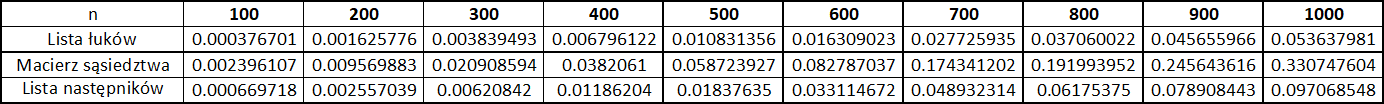
\includegraphics[width=1.0\linewidth]{luki_reprezentacje_tabela2}
\captionof{figure}{$d=0.4$ Zliczanie łuków z 3 reprezentacji - tabela}
\label{fig:luki_reprezentacje_tabela2}
\end{figure}%

Z wyników stworzyliśmy następujący wykres

\begin{figure}[h]
\centering
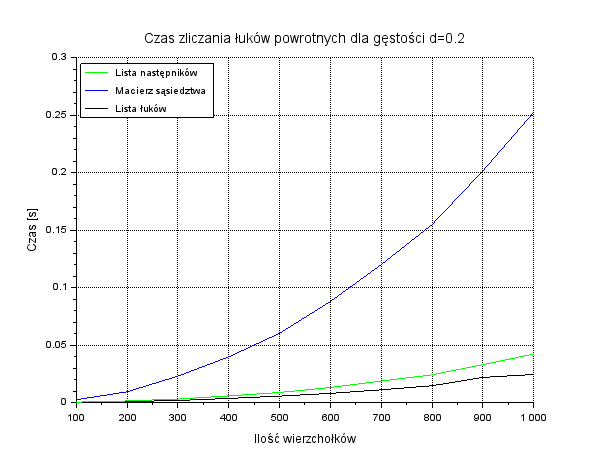
\includegraphics[width=0.5\linewidth]{luki_reprezentacje}
\captionof{figure}{$d=0.2$ Zliczanie łuków z 3 reprezentacji}
\label{fig:luki_reprezentacje}
\end{figure}%

\begin{figure}[h]
\centering
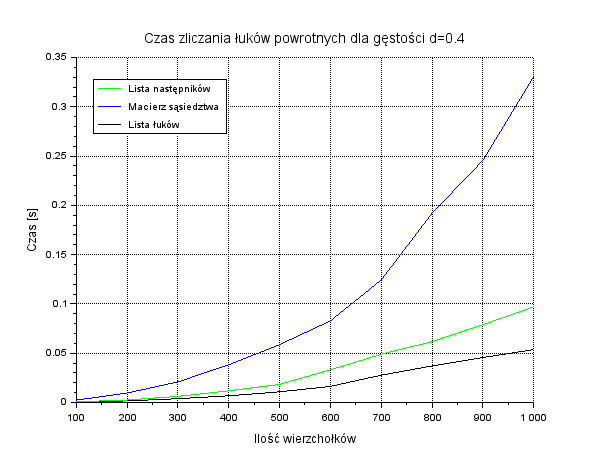
\includegraphics[width=0.5\linewidth]{luki_reprezentacje2}
\captionof{figure}{$d=0.4$ Zliczanie łuków z 3 reprezentacji}
\label{fig:luki_reprezentacje2}
\end{figure}%

Porównując ze sobą oba wykresy warto zauważyć, że czas wykonywania przy macierzy sąsiedztwa jest prawie taki sam, podczas gdy reprezentacje zależne od wartości $m$ doświadczają prawie dwukrotnego zwiększenia czasu operacji.

\section{Podsumowanie}

Wszystkie maszynowe reprezentacje grafów mają swoje wady i zalety - używając wiadomości poznanych w trakcie zajęć oraz doświadczeń wykonanych na potrzeby tego sprawozdania byliśmy w stanie sporządzić zbiór wad oraz zalet poznanych reprezentacji grafów.

Macierz sąsiedztwa ma dużą zaletę w postaci prostoty implementacji oraz małego obciążenia pamięci - pozwala ona na stworzenie macierzy bitowej i zajęcia znacznie mniejszej ilości pamięci. Ma ona również szybkie czasy sprawdzania poprzedników i następników mieszczące się w $O(n)$ oraz żadna jej operacja nie jest zależna od ilości łuków $m$. Wadą tej reprezentacji jest niepraktyczność w sytuacji małej gęstości grafu.

Macierze incydencji znajdują swoje najlepsze zastosowanie w hipergrafach, gdzie pojedyncza krawędź może być zbudowana z wielu połączeń - żadna inna poznana reprezentacja nie pozwala na przedstawienie tego w klarowny sposób. W przypadku rozpatrywanych w tym sprawozdaniu grafów ta reprezentacja wydaje się być najgorszą z poznanych - w grafie pełnym test wszystkich łuków zajmowałby czas rzędu aż $O(n^3)$.

Lista następników jest bardzo przydatna, kiedy zależy nam na szybkim wyszukiwaniu i analizowaniu następników, lub zbiorów następników - na przykład w algorytmie wyszukiwania "w głąb" omawianym wcześniej w tej pracy. Struktura jest prosta w implementacji w \textbf{python} oraz opłacalna przy niskich gęstościach - stanowi dobrą alternatywę dla macierzy sąsiedztwa podczas wykonywania DFS.

Lista poprzedników w funkcjonalności oferuje to samo co lista następników, z różnicą dotyczącą operacji sprawdzenia zbioru poprzedników - $O(n)$ i następników - $O(n+m)$. Dla listy następników złożoności tych operacji są "zamienione".

Lista łuków to dobra reprezentacja przy niskich wartościach $m$ pozwalająca na największe teoretyczne oszczędzenie pamięci zakładając małą gęstość grafu - jej główną zaletą jest zwracanie listy łuków w czasie $O(m)$ oraz wyszukiwanie binarne przy teście łuku w $O(\log m)$.

Wszystkie reprezentacje mają swoje wady oraz zalety i warto rozważyć wiele czynników podczas decydowania, która z nich jest lepsza do próby rozwiązania okazanego problemu.
\end{document}
